% !TEX root = cap01_standalone.tex
% Capítulo 1. Introducción
% Estructura según índice de la Dra. Lárraga.

\chapter{Introducción}
\label{ch:introduccion}

\section{Planteamiento del problema}

La superficie urbana del planeta crece más rápido que la población que la habita, y ese crecimiento se concentra en la periferia de las ciudades \parencite{Seto2012,UNHabitat2020,Angel2012}. La urbanización es un proceso social que transforma el territorio donde habita el ser humano, y el ritmo al que avanza rebasa la capacidad de los instrumentos que deberían ordenarla. De ahí la utilidad de anticipar qué suelo no urbano se convertirá en urbano: de ello depende que la vivienda y los servicios lleguen antes que la ocupación y no después.

Para responder esa pregunta se han desarrollado familias de modelos distintas. Los autómatas celulares son una de las más establecidas en el estudio del cambio de uso de suelo, porque representan el territorio como una rejilla de celdas cuyo estado evoluciona según reglas locales y explícitas. La vía que más se ha extendido en los últimos años consiste, en cambio, en aprender la regla de transición con redes neuronales. Esos modelos alcanzan ajustes satisfactorios, pero sus pesos no se dejan traducir a una pregunta geográfica, de modo que no puede afirmarse cuánto aportó cada variable a la transición de una celda concreta \parencite{almeida2008stochastic}; su aplicación en teledetección arrastra además la dificultad recurrente de conseguir datos etiquetados \parencite{Ma2019}. La distinción pesa cuando el destinatario del modelo es un instrumento de planeación, porque este necesita justificar sus decisiones y no solo acertarlas.

Al problema de la interpretabilidad se suma uno de datos. Evaluar un modelo de crecimiento urbano exige una serie de mapas comparables lo bastante larga para cubrir varios períodos, y esa serie rara vez está disponible para una ciudad concreta. La aplicación de escritorio de Google Earth ofrece una vía indirecta, pues su herramienta de imagen histórica permite recuperar la vista de una misma zona en distintos años. Lo que entrega, sin embargo, no son mapas: son capturas de pantalla en formato PNG, sin georreferencia y limitadas a las tres bandas del color visible, que hay que traducir a una clasificación urbano/no urbano antes de poder usarlas. El Capítulo~\ref{ch:modelo-crecimiento-urbano} describe esa fuente, la geometría que se recuperó de ella y los límites que impone.

La utilidad práctica de estos modelos depende de tres condiciones que rara vez se cumplen a la vez: que la regla de transición sea interpretable, que el desempeño se valide en más de un horizonte temporal y que el flujo completo sea reproducible con datos abiertos.

Estas tensiones se agudizan en las ciudades intermedias mexicanas, poco representadas en la literatura de modelado urbano: la revisión de \textcite{Wahyudi2016}, que clasifica por región ochenta y ocho aplicaciones de autómatas celulares urbanos, encuentra que al menos la mitad se concentra en ciudades de Estados Unidos y China, mientras que las de América del Sur son escasas. El Capítulo~\ref{ch:estado-del-arte} documenta ese vacío para el caso mexicano. La Zona Metropolitana de Querétaro sirve en este trabajo como caso de uso particular para ejercitar y validar el siguiente protocolo o algoritmo: una ciudad intermedia con una dinámica de expansión representativa y una serie de imágenes de archivo lo bastante larga para evaluarlo en varios períodos. Esto último tomará una gran relevancia al momento de definir por qué el diseño de la solución es correcto en términos de reproducibilidad y validación.

México tiene instrumentos de ordenamiento territorial, por ejemplo: la Ley General de Asentamientos
Humanos, los Programas Municipales de Ordenamiento Territorial y Desarrollo Urbano (PMOTDU),
la Secretaría de Desarrollo Agrario, Territorial y Urbano (SEDATU) y acuerdos con ONU-Hábitat.
Su cobertura efectiva es incompleta: la propia norma oficial mexicana en la materia registra
que solo $567$ municipios, el $22{,}94$\% del total, cuentan con un instrumento de
ordenamiento territorial o de desarrollo urbano, y que casi el $45$\% de esos instrumentos se
publicó hace más de quince años \parencite{SEDATU2024NOM005}. El INEGI documenta
que la mayor parte de la población reside en localidades urbanas \parencite{INEGI2020Censo}.
El resultado observable es un patrón de crecimiento disperso que supera la capacidad de
planificación disponible \parencite{ONUHabitat2016TendenciasMexico}, con impactos documentados sobre infraestructura, cobertura de
suelo y calidad de vida. Esos impactos están documentados en frentes distintos, de los que conviene mencionar algunos ejemplos: la
transformación de ecosistemas naturales en zonas urbanas contribuye a la pérdida de
hábitat, señalada como la principal causa de pérdida de biodiversidad en el
país \parencite{CONABIO2024Porque}. El transporte terrestre que la dispersión convierte en necesario tiene externalidades negativas documentadas para el caso
mexicano \parencite{ITDP2019Externalidades}. Y los efectos del cambio de suelo urbano no
se agotan en el área que se urbaniza: alcanzan a los territorios con los que la ciudad se
conecta mediante flujos de personas, bienes y capital \parencite{Seto2012teleconnections}.

\begin{figure}[htbp]
\centering
\begin{subfigure}[b]{0.32\textwidth}
	\centering
	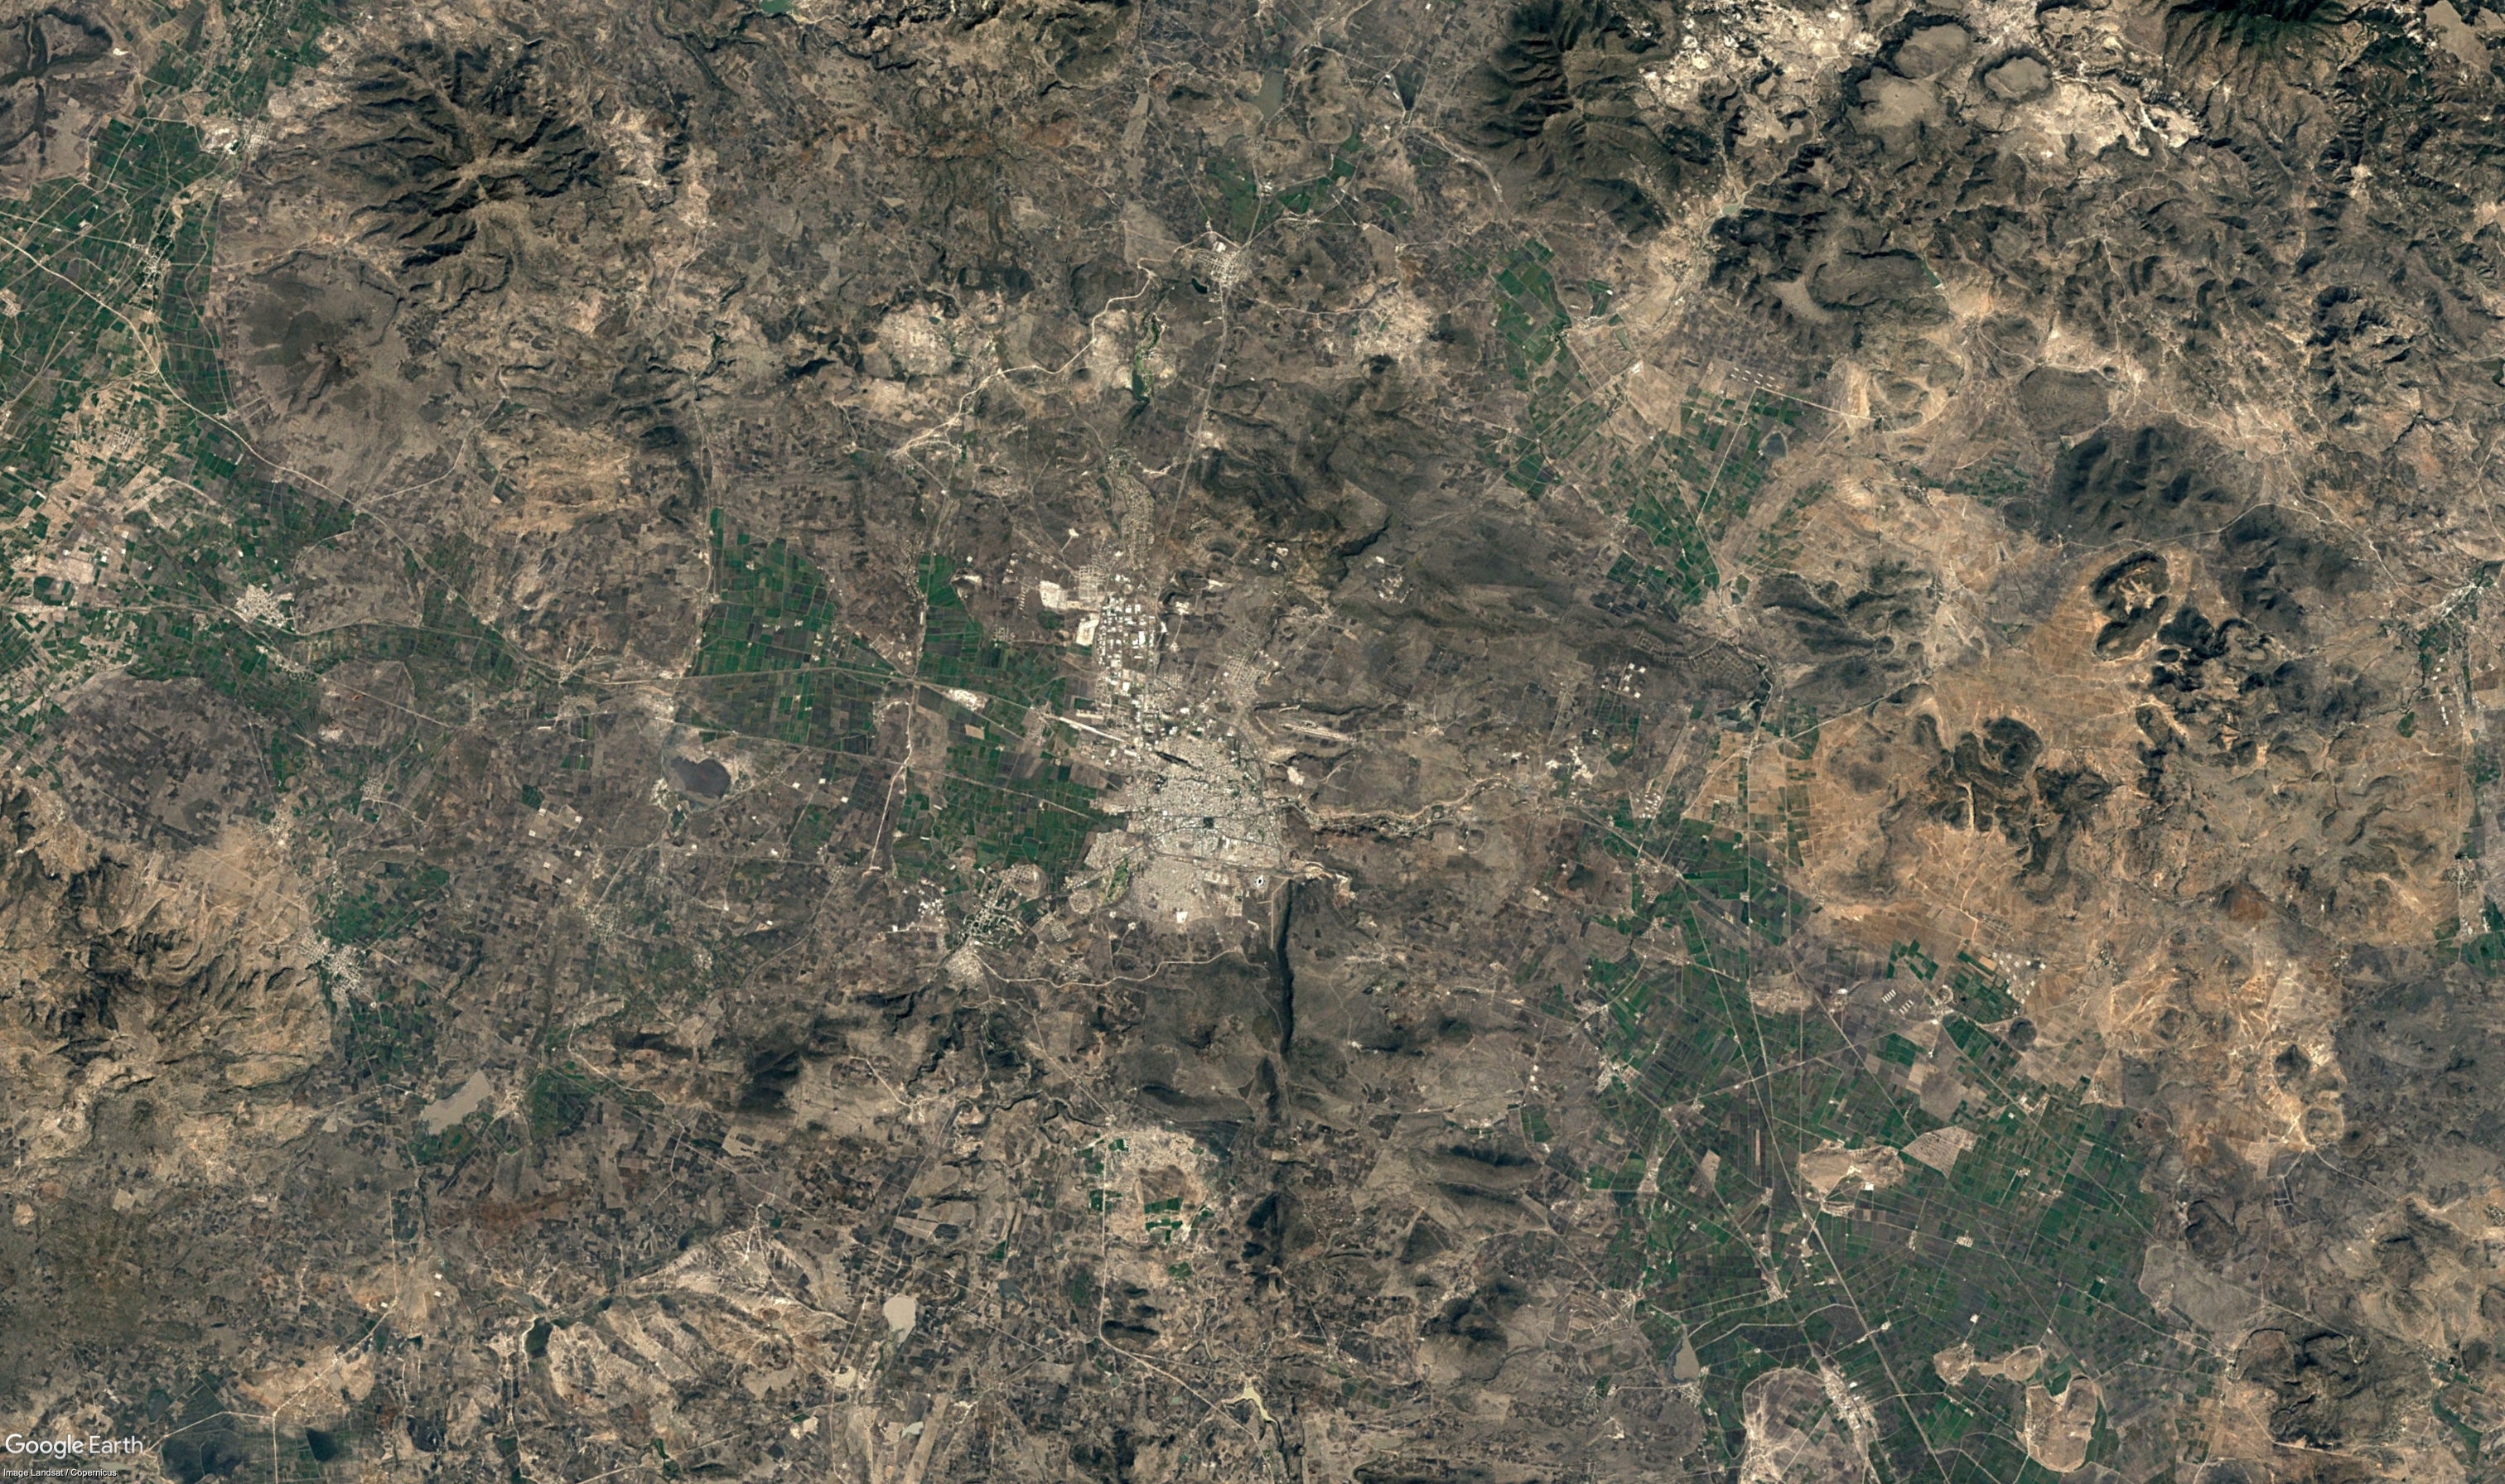
\includegraphics[width=\textwidth]{figures/raw_capture_zmq_1984.png}
	\caption{1984}
	\label{fig:raw_zmq_1984}
\end{subfigure}
\hfill
\begin{subfigure}[b]{0.32\textwidth}
	\centering
	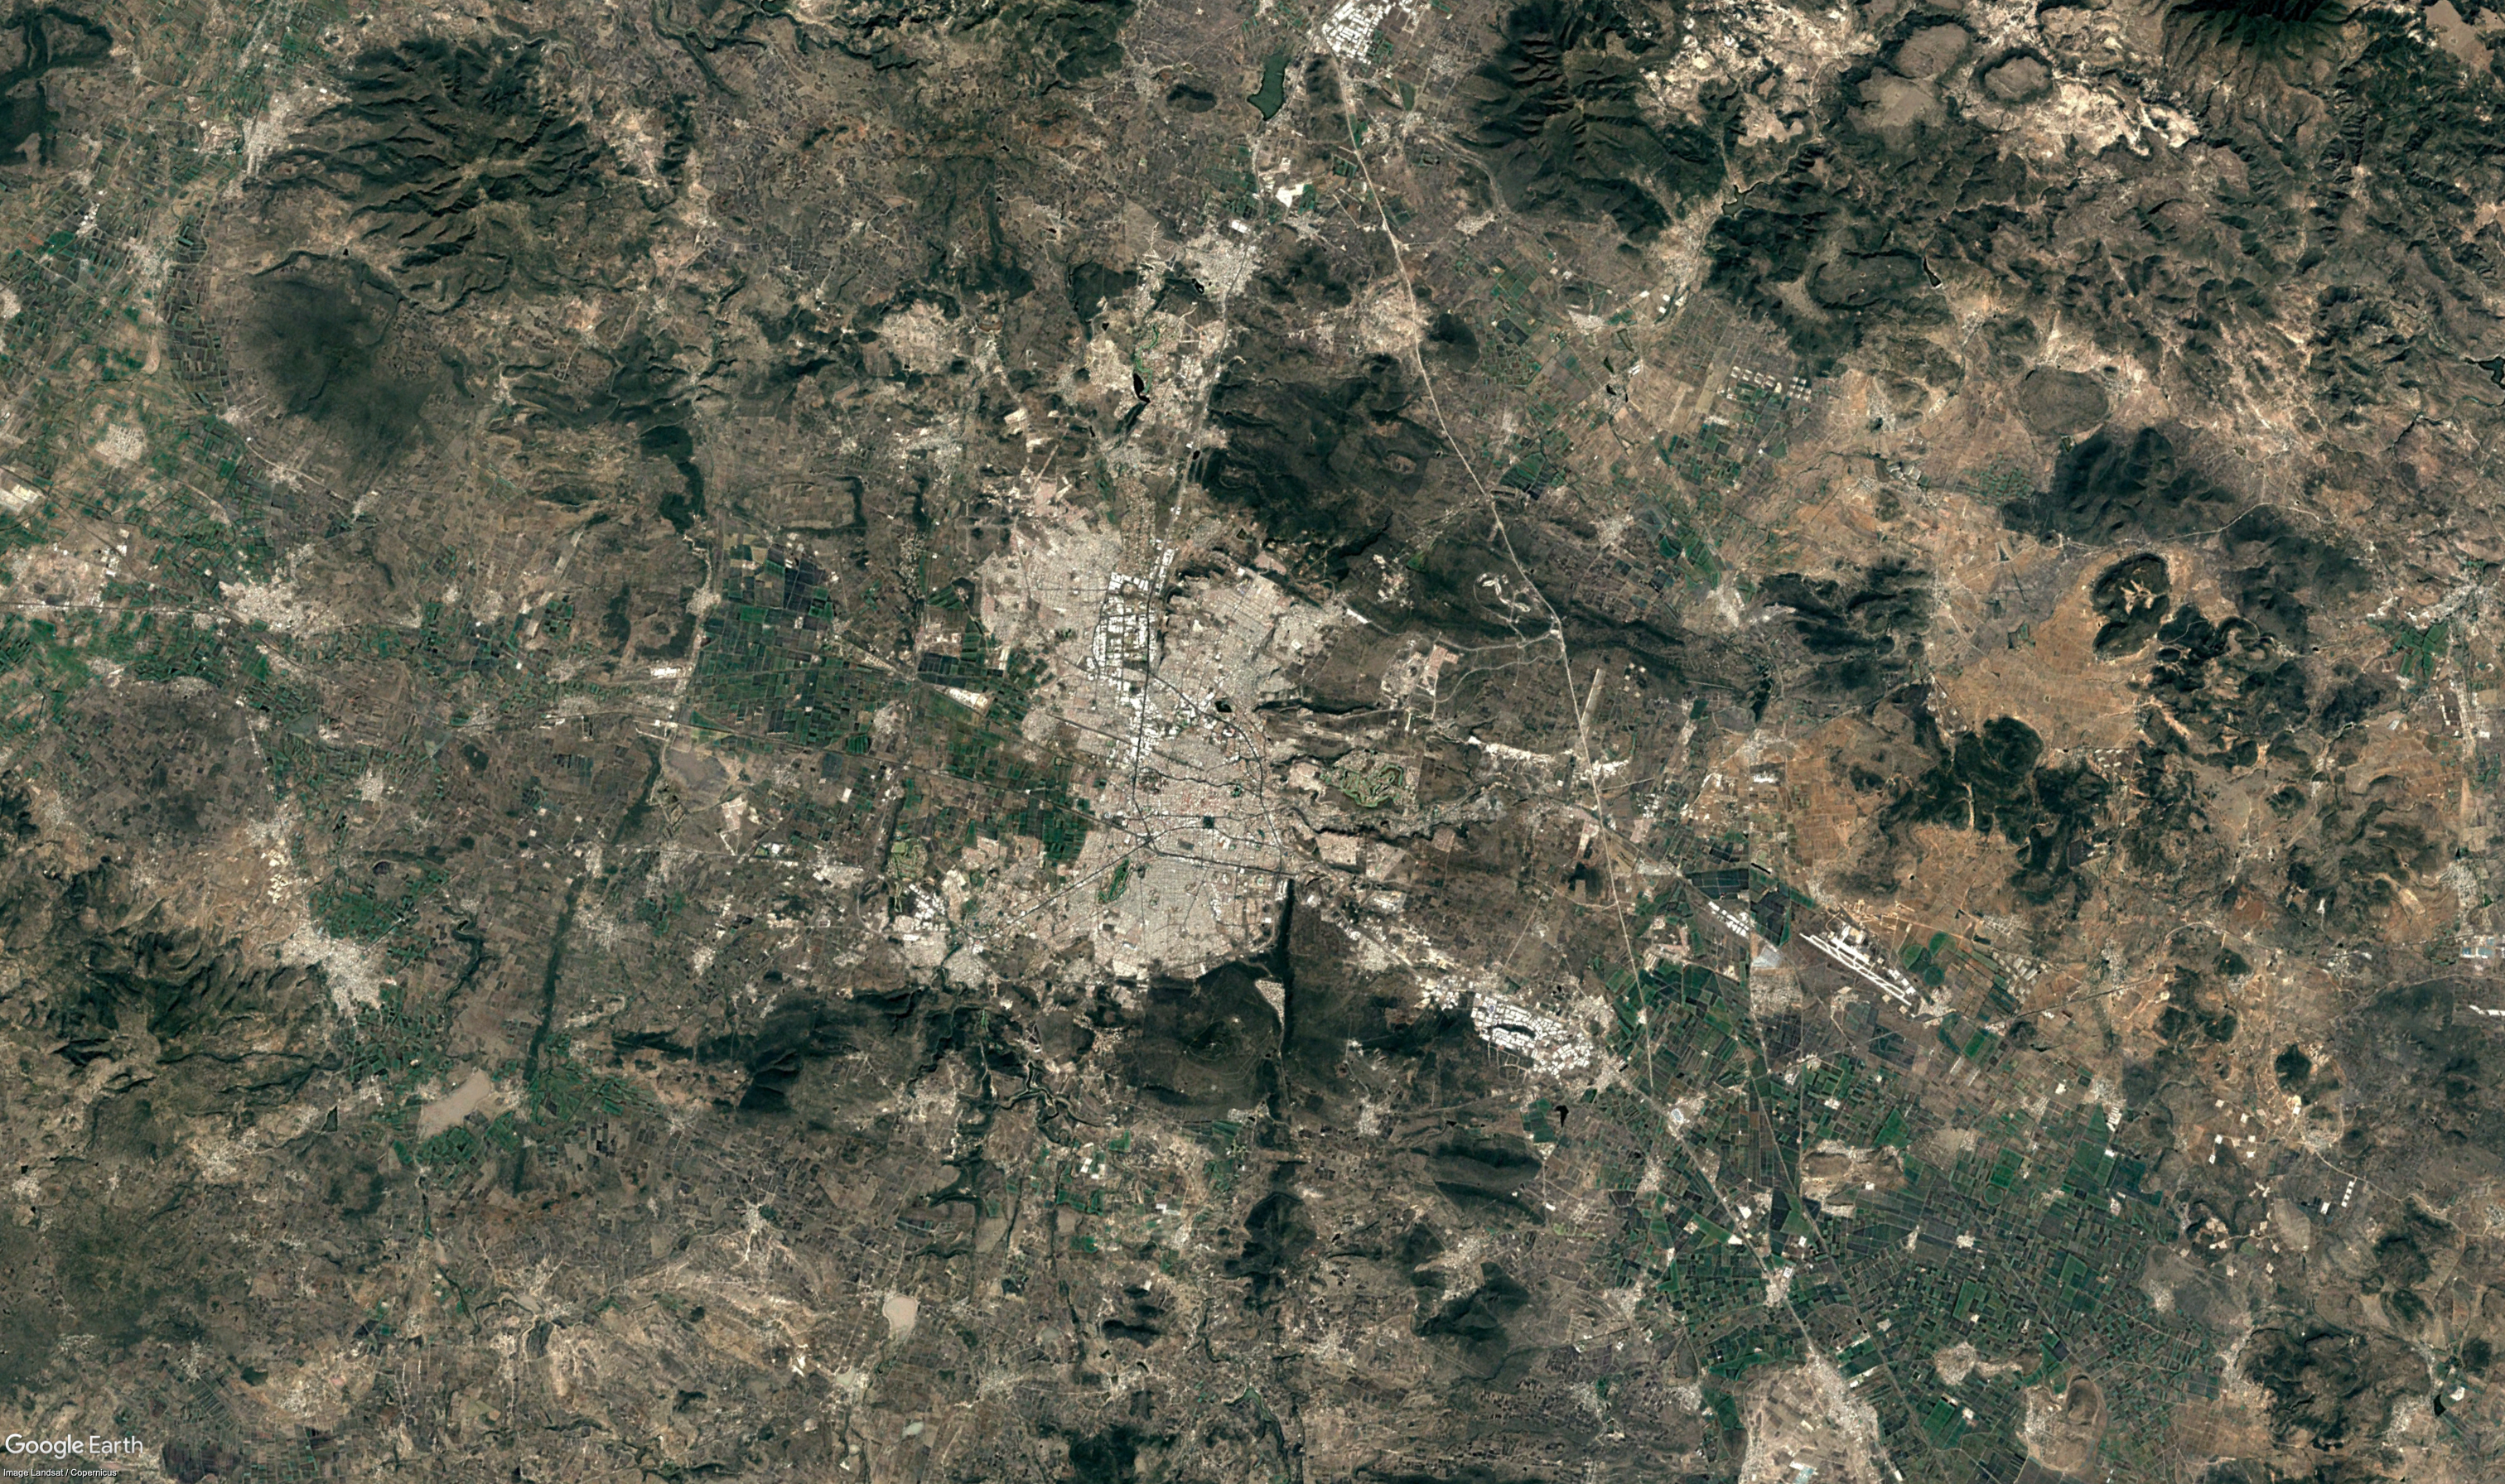
\includegraphics[width=\textwidth]{figures/raw_capture_zmq_2010.png}
	\caption{2010}
	\label{fig:raw_zmq_2010}
\end{subfigure}
\hfill
\begin{subfigure}[b]{0.32\textwidth}
	\centering
	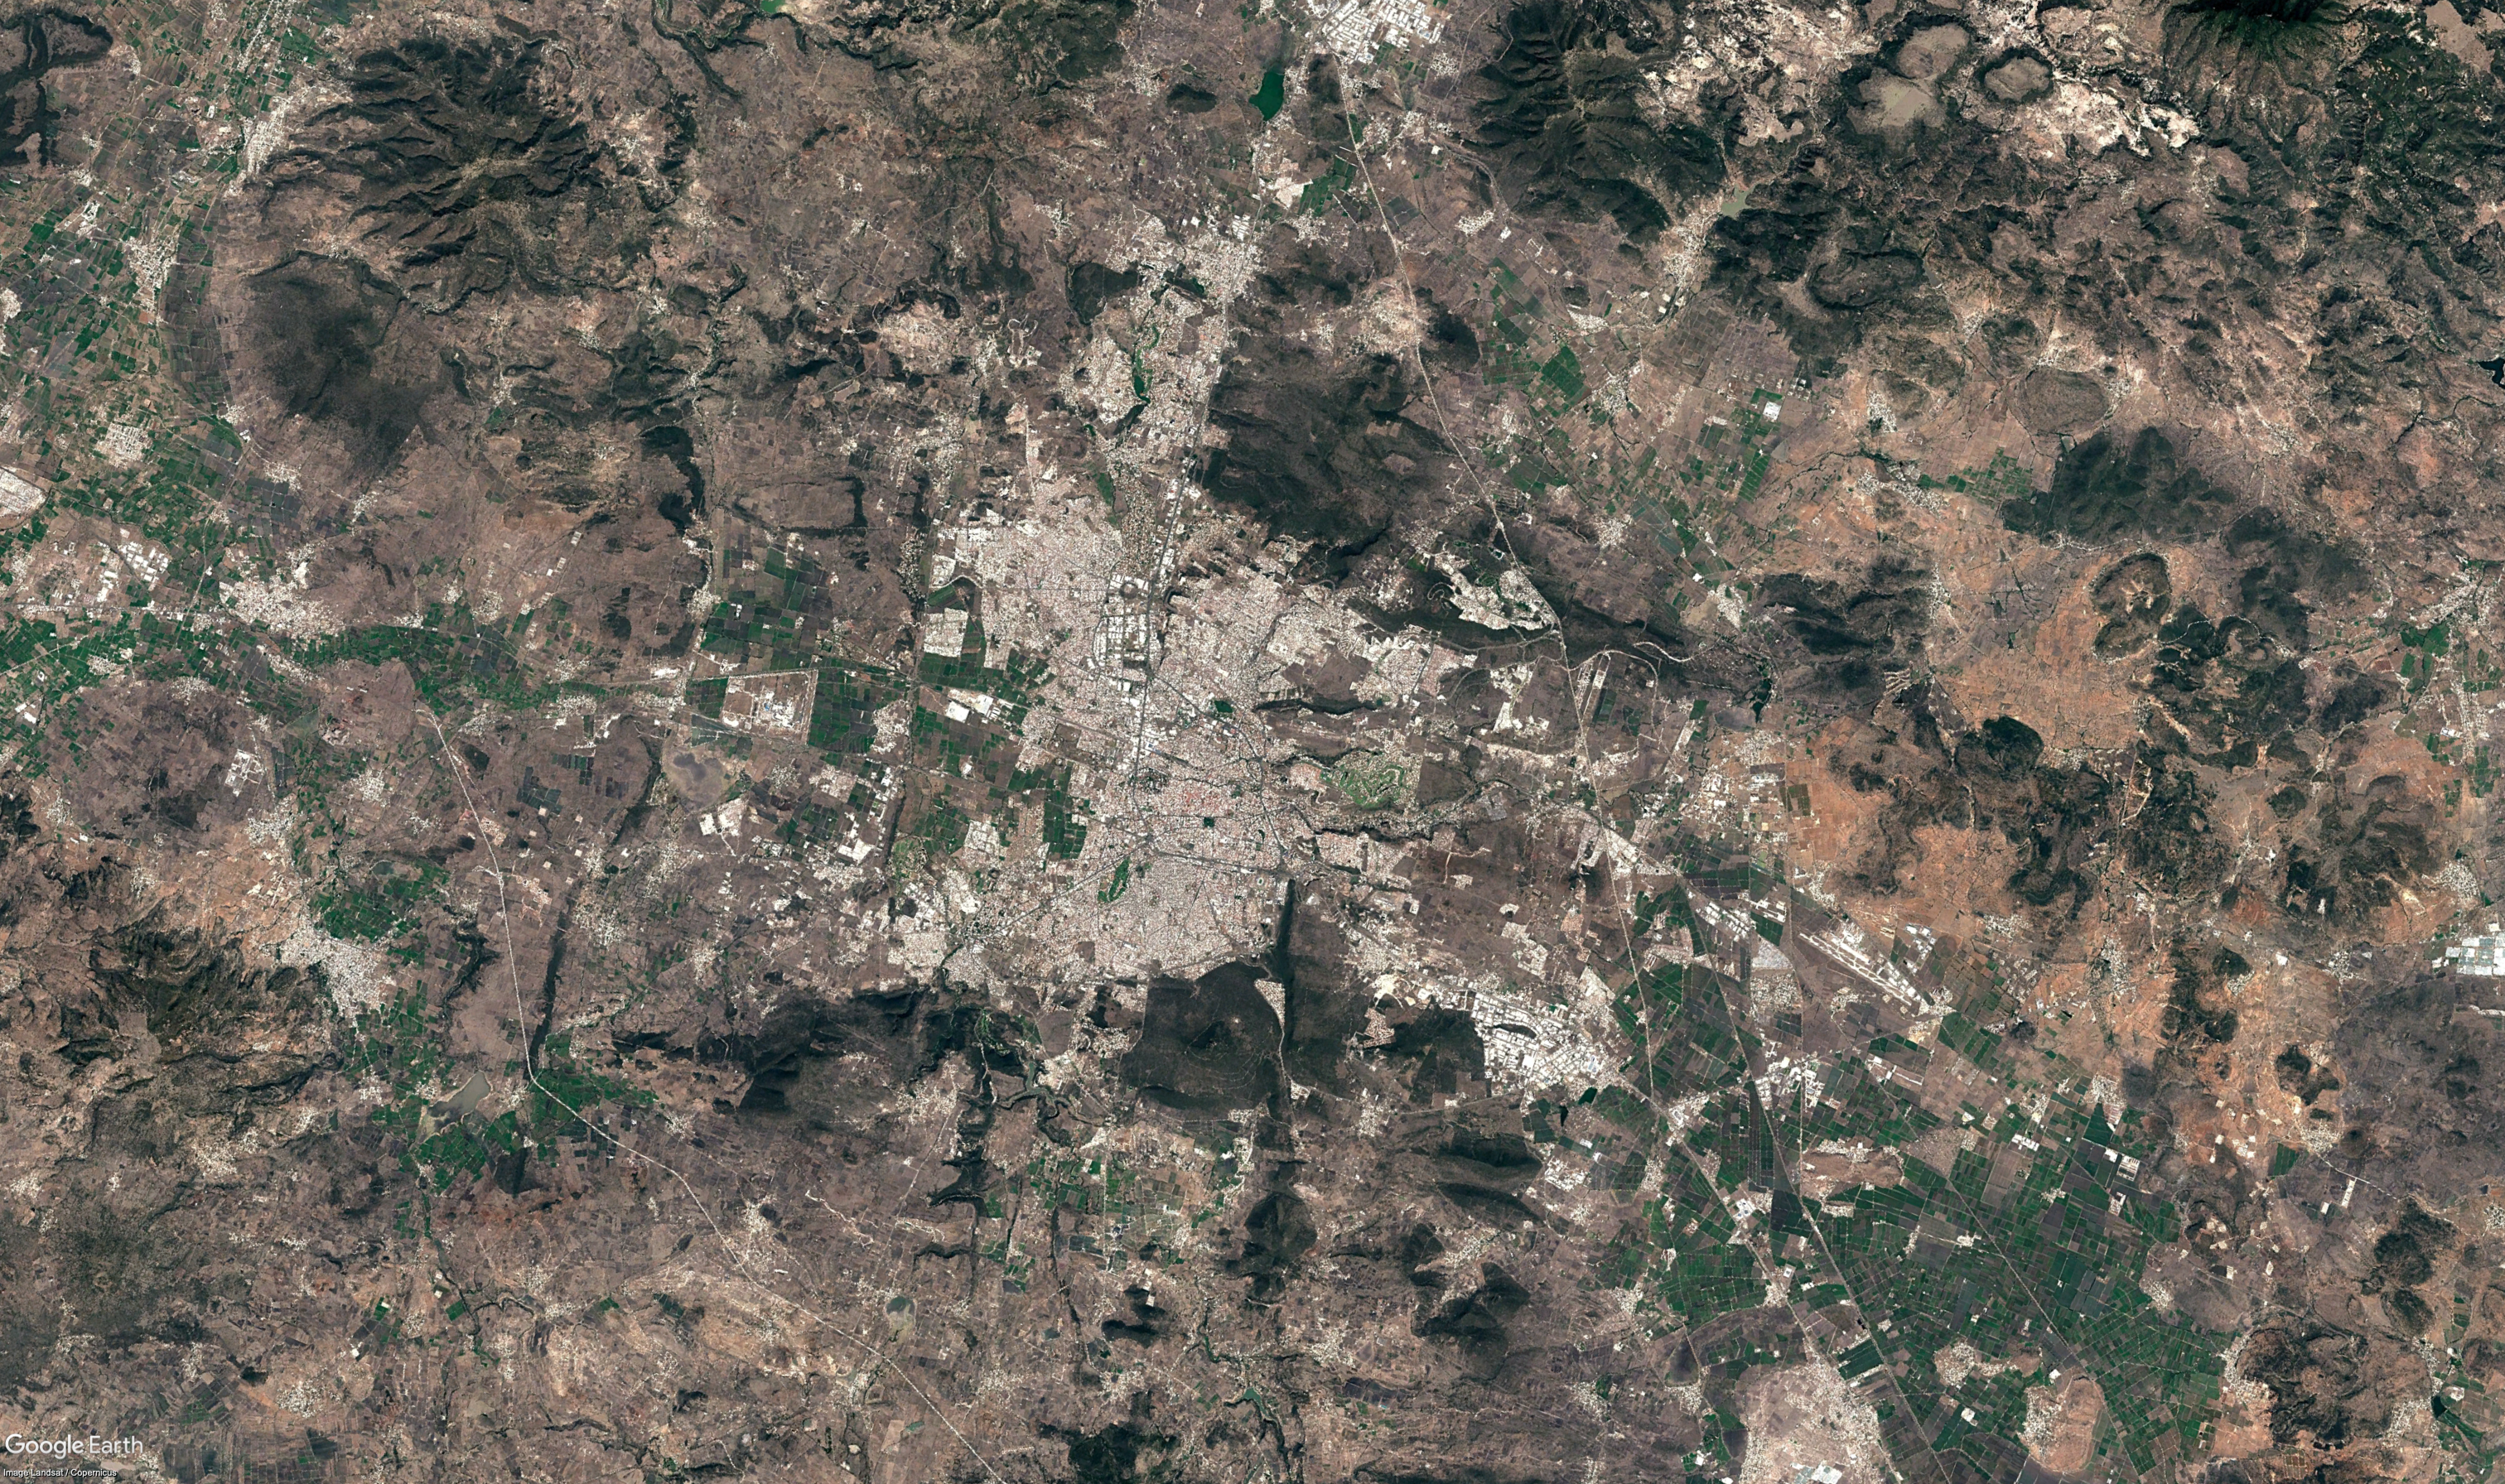
\includegraphics[width=\textwidth]{figures/raw_capture_zmq_2020.png}
	\caption{2020}
	\label{fig:raw_zmq_2020}
\end{subfigure}
\caption{Secuencia de \textbf{capturas RGB} (insumo \textit{raw}) obtenidas con Google Earth en modo imagen histórica sobre la Zona Metropolitana de Querétaro (\textbf{1984}, \textbf{2010} y \textbf{2020}), en orden cronológico y con encuadre homogéneo según el procedimiento manual descrito para la serie temporal. Visualmente se aprecia la expansión periférica y un patrón de ocupación predominantemente disperso.}
\label{fig:crecimiento_disperso_zmq_1984_2020}
\end{figure}

Como se observa en la figura~\ref{fig:crecimiento_disperso_zmq_1984_2020}, la mancha
urbana de Querétaro se expandió de forma dispersa entre 1984 y 2020, sobre una zona
metropolitana que rebasó el millón y medio de habitantes en el censo de 2020
\parencite{INEGI2020Censo}, tras décadas de expansión sostenida a una tasa media anual
del $2{,}8$\% \parencite{CONAPO2018Delimitacion}. 

Ese patrón se ha documentado para Querétaro en relación con la producción de vivienda
\parencite{ObservatorioCiudades2022Queretaro}, e impide anticipar dónde y a qué velocidad se
producirá la siguiente oleada de expansión: información necesaria para planear el uso de
recursos y la infraestructura que el crecimiento urbano demanda.

Como instancia
concreta de este problema, la predicción del crecimiento urbano, el trabajo implementa la solución usando el modelo que integra autómatas celulares con pesos de evidencia y con validaciones multitemporales sobre un conjunto de datos enriquecidos sobre la ZMQ. Para que un modelo de simulación sea útil como herramienta
de apoyo a la planeación, debe satisfacer los cuatro requerimientos de la
Tabla~\ref{tab:requerimientos_modelo_1}.

\begin{table}[H]
	\centering
	\caption{Requerimientos del modelo de crecimiento urbano para la ZMQ.}
	\label{tab:requerimientos_modelo_1}
	\begin{tabularx}{\textwidth}{c >{\raggedright\arraybackslash}p{3.3cm} >{\raggedright\arraybackslash}X}
	\toprule
	\textbf{ID} & \textbf{Requerimiento} & \textbf{Descripción y criterio de cumplimiento} \\
	\midrule
	R1 & Simulación histórica con precisión &
	Reproducir el patrón de cambio urbano/no-urbano a partir del historial de uso de suelo.
	El desempeño se evalúa cuantitativamente con \textit{Figure of Merit} (FoM), Kappa e
	\textit{Intersection over Union} (IoU) en ventanas de validación
	desplazadas respecto del entrenamiento. \\
	\addlinespace
	R2 & Soporte a planeación estratégica &
	Generar mapas espacialmente explícitos que sirvan para comparar patrones de expansión
	bajo supuestos declarados, leídos como escenarios y no como planes calibrados. \\
	\addlinespace
	R3 & Replicabilidad y apertura &
	El procesamiento debe ser documentado, reproducible y ejecutable sin software propietario
	ni hardware especializado, con calibración sistemática y tiempos de cómputo razonables. \\
	\addlinespace
	R4 & Interpretabilidad de la función de transición &
	La función que decide la transición de cada celda debe ser auditable: sus pesos deben ser
	legibles como evidencia espacial cuantificable, no como parámetros opacos de una red
	neuronal. \\
	\bottomrule
	\end{tabularx}
\end{table}

\section{Justificación}

En cualquier ciudad es poco frecuente disponer de un modelo que simule y haga predicción sobre el crecimiento de dicha ciudad en el tiempo, que aparte sea validado en varios horizontes de tiempo, que sea transparente en la forma en la que modela así como que sea reproducible con datos abiertos. Mientras esta brecha persista, no es posible distinguir si los modelos existentes responden a mecanismos espaciales estables o un sobreajuste. Los requerimientos R1--R4 de la Tabla~\ref{tab:requerimientos_modelo_1} son la forma operativa de comprobar si un modelo cierra esa brecha.

\section{Antecedentes}

El modelado del crecimiento urbano cuenta con muchos estudios, que pueden agruparse según el tipo de función de transición que implementan. Los modelos de caja negra basados en aprendizaje automático \parencite{almeida2008stochastic,Gomez2020} aprenden la función de transición de los datos sin imponerle una forma previa, pero sus pesos internos no son legibles como evidencia espacial, lo que dificulta su uso en contextos que exigen transparencia metodológica. Por otro lado, los metaheurísticos \parencite{Wang2021} persiguen la configuración urbana que optimiza una función objetivo definida por el analista, de modo que responden a una pregunta normativa y no predictiva; la calibración por búsqueda sobre el espacio de parámetros puede además resultar costosa, como documenta \textcite{Jantz2003} para SLEUTH, donde el ajuste tomó más de una semana de cómputo en un clúster de dieciséis nodos. Los modelos de caja blanca más citados \parencite{Clarke1998}, y las revisiones que los sistematizan \parencite{Sante2010,Aburas2016}, atienden la interpretabilidad, pero la práctica de validación del campo es endeble: en una revisión de aplicaciones recientes de modelos de cambio de suelo, el 31\% no reporta validación alguna y el resto se apoya predominantemente en la exactitud locacional frente a un solo mapa observado \parencite{vanVliet2016}. Con una sola comparación no es posible determinar si el desempeño refleja mecanismos espaciales estables o sobreajuste a esa fase concreta del crecimiento.

Los trabajos representativos para ciudades mexicanas \parencite{SuarezDelgado2007,RamirezHernandez2021,Chihuahua2023} cumplen R2 y, en distinto grado, R4; ninguno cumple R3 y solo uno de ellos satisface R1 de forma parcial. Las aplicaciones basadas en Pesos de Evidencia se han calibrado y validado principalmente en contextos internacionales, con dinámicas de crecimiento y fuentes de datos distintas a las ciudades intermedias del país. El análisis detallado de estos trabajos se desarrolla en el Capítulo~\ref{ch:estado-del-arte}.

El proyecto presente diseñó e implementó la validación de un modelo que acopla Pesos de Evidencia con Autómatas Celulares para simular el crecimiento urbano para un caso particular de la Zona Metropolitana de Querétaro en el período 1984-2020, evaluar su desempeño mediante métricas espaciales cuantitativas a lo largo de cinco ventanas quinquenales desplazadas y comparar los resultados con valores de referencia reportados en la literatura.

\section{Objetivos}

\subsection{Objetivo general}

Diseñar e implementar un modelo utilizando autómatas celulares con pesos de evidencia y con validaciones multitemporales sobre un conjunto de datos. En particular se validó el modelo con el caso de uso de la Zona Metropolitana de Querétaro en el período 1984--2020. Este modelo debe cumplir con los requerimientos R1--R4 de la Tabla~\ref{tab:requerimientos_modelo_1} y debe ser capaz de simular auditablemente el crecimiento urbano de la ciudad de Querétaro en el período 1984--2020.

\subsection{Objetivos específicos}

El primer objetivo específico (OE1) consiste en construir una serie histórica anual
(1984--2020) de mapas binarios urbano/no-urbano para la ZMQ a partir de imágenes de
archivo de Google Earth, empleando clasificación no supervisada para prescindir de
etiquetas manuales, de modo que el flujo de adquisición y preprocesamiento sea
cuyo procesamiento es replicable sin software propietario. Sobre esa serie, el segundo objetivo (OE2) selecciona y
calcula las variables espaciales derivadas de los mapas binarios, que sirven de evidencia
empírica al modelo WoE. La elección de WoE como función de transición, frente a
alternativas como la regresión logística o las redes neuronales, responde a su capacidad
de descomponer la contribución de cada variable mediante el \textit{Information Value} (IV),
propiedad que hace auditable la decisión celda a celda y cumple el requerimiento R4 de la
Tabla~\ref{tab:requerimientos_modelo_1}.

El tercer objetivo (OE3) diseña e implementa el autómata celular WoE-AC que simula la transición
de no urbano a urbano en la ZMQ. La decisión de usar AC sobre enfoques basados en agentes
(ABM), que exigen declarar el comportamiento de cada
agente \parencite{Li2007}, o modelos estadísticos puros se fundamenta en que los AC
capturan la dinámica de
difusión espacial emergente sin requerir la especificación de reglas de comportamiento
individual, y mantienen la interpretabilidad del modelo al nivel de la rejilla espacial
\parencite{Clarke1998,Sante2010,Batty2005}. El cuarto objetivo (OE4) calibra sistemáticamente los
parámetros del WoE-AC (umbral de transición y peso de vecindad) mediante búsqueda en
cuadrícula y establece un protocolo de validación multi-período con cinco ventanas
quinquenales desplazadas (2011--2016 a 2015--2020), evaluadas con FoM, Kappa e IoU. La
\textcite{pontius2008comparing} documentan que las aplicaciones con mayor cambio neto
observado tienden a obtener un FoM más alto, de modo que un único horizonte no permite separar
el mérito del modelo del de la fase de crecimiento medida. La validación en ventanas
desplazadas responde a esa dependencia: al repetir la evaluación sobre cinco períodos, un
desempeño sostenido no puede atribuirse a una sola fase.

Por último, el quinto objetivo (OE5) analiza la estabilidad temporal del desempeño del modelo a
lo largo de los cinco períodos y compara los valores de FoM e IoU obtenidos con los rangos
reportados en la literatura para modelos de caja blanca y de caja negra, con el fin de
posicionar la contribución del trabajo en el contexto del estado del arte.

\section{Preguntas de investigación e hipótesis}

\subsection{Preguntas de investigación}

La investigación se articula en torno a cuatro preguntas, que se identifican como P1 a P4
para poder rastrear su respuesta en las conclusiones. \textbf{P1} indaga si un modelo
WoE-AC calibrado puede reproducir el patrón de crecimiento urbano observado en la Zona
Metropolitana de Querétaro (ZMQ) con métricas espaciales (Figure of Merit, Kappa e
Intersection over Union) comparables a las de la literatura. \textbf{P2} interroga qué
variables espaciales tienen mayor poder discriminatorio para predecir la transición urbana
en la ZMQ. \textbf{P3} examina si el modelo mantiene la estabilidad de su desempeño al
evaluarse en cinco ventanas quinquenales desplazadas (2011--2016 a 2015--2020). Cada
ventana queda fuera del entrenamiento; entre sí se solapan. \textbf{P4} plantea si el flujo
completo, desde la adquisición de imágenes hasta la validación, se ejecuta con herramientas
de código abierto en una CPU estándar, sin GPU ni software propietario, una vez disponibles las capturas.

\subsection{Hipótesis}

\textbf{Hipótesis general.} Un modelo híbrido WoE-AC, calibrado y validado mediante un protocolo multitemporal sobre datos de libre acceso, permite simular de forma interpretable y reproducible el crecimiento urbano de una ciudad intermedia mexicana con un desempeño comparable al reportado en la literatura.

De esa hipótesis general se derivan cuatro particulares, cada una falsable con los resultados del Capítulo~\ref{ch:resultados-analisis}.

\textbf{H1 (interpretabilidad).} La regla de transición basada en WoE ponderada por Information Value produce un modelo en el que cada variable contribuye de forma auditable: la distancia al frente urbano y la densidad de vecindad concentran el mayor IV, por encima de las variables de fragmentación y de gradiente.

\textbf{H2 (estabilidad temporal).} El desempeño del modelo se sostiene en cinco ventanas quinquenales desplazadas (2011--2016 a 2015--2020), sin degradación sistemática atribuible al modelo. El valor más bajo se asocia a la ventana de menor crecimiento neto observado, no a un fallo de calibración.

\textbf{H3 (reproducibilidad).} El procesamiento completo, desde las capturas hasta la validación quinquenal, se ejecuta con herramientas de código abierto en una CPU estándar, sin requerir GPU, software propietario ni hardware especializado. La adquisición de las imágenes depende del visor de Google Earth, que no es de código abierto; esa es la única dependencia externa del flujo y se documenta como tal.

\textbf{H4 (desempeño comparable).} Aplicado a la Zona Metropolitana de Querétaro, el modelo reproduce el patrón de crecimiento con un FoM por encima del subconjunto de aplicaciones con FoM inferior a $0{,}15$ del espectro multi-sitio de \textcite{pontius2008comparing}, acompañado de valores de Kappa e IoU sostenidos en los cinco períodos, sin recurrir a representaciones de caja negra.

% La sección "Alcances y limitaciones" se trasladó al capítulo de conclusiones
% (orden exigido: Alcances -> Limitaciones -> Trabajo futuro).

\section{Aportaciones del trabajo}

La combinación de Pesos de Evidencia y autómatas celulares no es, en sí misma, una novedad
metodológica: existe una literatura consolidada que la emplea. Lo que distingue a este
trabajo no es la técnica, sino la metodología con que se evaluó y las condiciones de
reproducibilidad bajo las que se aplicó.

La principal aportación es de carácter metodológico, con un proceso de evaluación reproducible y multiperíodo. En vez de validar sobre un solo horizonte temporal, el modelo se evaluó sobre cinco ventanas quinquenales con un conjunto de métricas espaciales que se complementan entre sí, a saber el Figure of Merit, Kappa e Intersection over Union, así como la descomposición del error de Pontius entre desacuerdo de cantidad y de asignación, situando
el desempeño en el espectro empírico multi-sitio de referencia. Ese protocolo permite
distinguir un desempeño estable de un ajuste a una fase concreta del crecimiento, y arrojó
métricas dentro del rango reportado en la literatura (FoM promedio $0{,}317$, Kappa promedio
$0{,}445$), sostenidas a lo largo de los cinco horizontes y no concentradas en uno solo.

Sobre ese núcleo se apoyan las demás aportaciones. El flujo completo, desde la adquisición de
imágenes hasta la validación quinquenal, se implementó con herramientas de código abierto y
quedó documentado paso a paso, de modo que otros investigadores puedan reproducirlo,
adaptarlo o extenderlo a otras ciudades intermedias. La función de transición WoE aporta,
además, pesos de evidencia y valores de información (IV) legibles por variable, lo que mantiene auditable cada
decisión del modelo y facilita interpretar los resultados en términos de los mecanismos
espaciales que los sustentan.

El protocolo se ejercita, por último, sobre un contexto poco representado en la literatura de
modelado urbano: las ciudades intermedias mexicanas, habitualmente analizadas con
calibraciones heurísticas y sobre un solo horizonte temporal. Para ello se construyó una
serie histórica larga, 37 años continuos (1984--2020), a partir de imágenes de archivo de
acceso libre. Esa base es más extensa que la de los trabajos comparables para el país
revisados en la Sección~\ref{sec:vacios-mexico}, que operan sobre ventanas de diez años
\parencite{SuarezDelgado2007}, veinte \parencite{RamirezHernandez2021}, catorce
\parencite{JimenezLopez2018} y cinco \parencite{Chihuahua2023}. Querétaro es el caso de uso donde el protocolo se ejercita y se valida.

\section{Organización del documento}

El resto de la tesis sigue el hilo que abre este diagnóstico. El Capítulo~\ref{ch:marco-teorico} fija el andamiaje formal mínimo (fundamentos del preprocesamiento de imágenes, autómatas celulares probabilísticos, Pesos de Evidencia y métricas de evaluación espacial) que el modelo necesita para ser especificado y evaluado con precisión. El Capítulo~\ref{ch:estado-del-arte} muestra que los problemas metodológicos que motivan el trabajo (calibración heurística, validación en un solo período, dependencia de plataformas de código cerrado y poca presencia de ciudades intermedias mexicanas en la literatura) siguen abiertos y justifican la propuesta. El Capítulo~\ref{ch:modelo-crecimiento-urbano} es el núcleo empírico: presenta el área de estudio, los datos y su preprocesamiento, y formaliza el acoplamiento WoE-AC, su calibración por búsqueda sistemática y el protocolo de validación quinquenal múltiple. El Capítulo~\ref{ch:resultados-analisis} muestra que el modelo se sostiene en las cinco ventanas (FoM medio $0{,}317$) y lo sitúa frente a la literatura. Por último, el Capítulo~\ref{ch:conclusiones} contrasta las hipótesis con la evidencia, precisa las aportaciones, define los alcances y acota lo que el modelo sí y no permite afirmar, junto con las líneas de trabajo futuro. El Apéndice~\ref{ap:arquitectura} reúne el material de soporte: la arquitectura de software, el pseudocódigo del pipeline de clasificación y las tablas de detalle de las características y del preprocesamiento.
